\documentclass[11pt]{article}

%% PACKAGES
\usepackage{graphicx}
\usepackage[printonlyused]{acronym}
\usepackage{float}
\usepackage[colorlinks=false]{hyperref}
\usepackage{tabularx}
\usepackage{caption}
\usepackage[margin=1.0in]{geometry}
\usepackage{tocloft}
\usepackage{listings}

\lstset{basicstyle=\small\ttfamily,columns=flexible,breaklines=true,xleftmargin=0.5in,keepspaces=true}


\makeatletter
\g@addto@macro\normalsize{%
  \setlength\abovedisplayskip{0.25pt}
  \setlength\belowdisplayskip{0.25pt}
  \setlength\abovedisplayshortskip{0.25pt}
  \setlength\belowdisplayshortskip{0.25pt}
}
\makeatother

\setlength{\parskip}{\baselineskip}

%% GRAPHICS PATH
\graphicspath{{../../shared_latex_inputs/images}{../../shared_latex_inputs/graphs}}

\newcommand{\acposs}[1]{%
	\expandafter\ifx\csname AC@#1\endcsname\AC@used
	\acs{#1}'s%
	\else
	\aclu{#1}'s (\acs{#1}'s)%
	\fi
}

\title{\Huge EMTG Testatron Tutorial: Creating a Test}

\newcommand{\listofknownissuesname}{\Large List of Known Issues}
\newlistof{knownissues}{mcf}{\listofknownissuesname}

\newcommand{\knownissue}[3]
{
	\refstepcounter{knownissues}
	\par\noindent\textbf{\hyperref[#2_b]{\theknownissues\quad #1}}\label{#2_h}
	\textbf{\hfill\pageref{#2_b}}
	#3
}

\newcommand{\knownissuelabel}[2]
{
	 \phantomsection
  	\hyperref[#2_h]{#1}\def\@currentlabel{\unexpanded{#1}}\label{#2_b}
}


\begin{document}

\begin{titlepage}
\maketitle
\thispagestyle{empty}
\begin{table}[H]
	\centering
	\begin{tabularx}{\textwidth}{|l|l|X|}
		\hline
		\textbf{Revision Date} & \textbf{Author} & \textbf{Description of Change} \\
		\hline
		\date{June 30, 2023} & Joseph Hauerstein & Initial revision.\\ 
		\hline
	\end{tabularx}
\end{table}
\end{titlepage}

\newpage
\tableofcontents
\thispagestyle{empty}
\newpage

\listofknownissues
\thispagestyle{empty}

\knownissue{Testatron does not update the paths of files in HardwareModels.}{hardware_options_file_paths_issue}

\knownissue{The output produced by running Testatron is different from PyEMTG.}{testatron_changes_emtgopt_issue}

\newpage
\clearpage
\setcounter{page}{1}



\section*{List of Acronyms}
\begin{acronym}
%To define the acronym and include it in the list of acronyms: \acro{acronym}{definition}
%To define the acronym and exclude it from the list of acronyms:  \acro{acronym}{definition}
%
%\ac{acronym} Expand and identify the acronym the first time; use only the acronym thereafter
%\acf{acronym} Use the full name of the acronym.
%\{acronym} Use the acronym, even before the first corresponding \ac command
%\acl{acronym}  Expand the acronym without using the acronym itself.
%
%

\acro{ACS}{attitude control system}
\acro{ACO}{Ant Colony Optimization}
\acro{AD}{Automatic Differentiation}
\acro{ADL}{Architecture Design Laboratory}
\acro{AES}{Advanced Exploration Systems}
\acro{AGA}{aerogravity assist}
\acro{ALARA}{As Low As Reasonably Achievable}
\acro{API}{application programming interface}
\acro{BB}{branch and bound}
\acro{BVP}{Boundary Value Problem}
\acro{CATO}{Computer Algorithm for Trajectory Optimization}
\acro{CL}{confidence level}
\acro{CONOPS}{concept of operations}
\acro{COV}{Calculus of Variations}
\acro{D/AV}{Descent/Ascent Vehicle}
\acro{DE}{Differential Evolution}
\acro{DLA}{Declination of Launch Asymptote}
\acro{RLA}{Right Ascension of Launch Asymptote}
\acro{RA}{right ascension}
\acro{DEC}{declination}
\acro{DPTRAJ/ODP}{Double Precision Trajectory and Orbit Determination Program}
\acro{DSH}{Deep Space Habitat}
\acro{DSN}{Deep Space Network}
\acro{DSMPGA}{Dynamic-Size Multiple Population Genetic Algorithm}
\acro{EB}{Evolutionary Branching}
\acro{ECLSS}{environmental control and life support system}
\acro{ELV}{expendable launch vehicle}
\acro{EMME}{Earth to Mars, Mars to Earth}
\acro{EMMVE}{Earth to Mars, Mars to Venus to Earth}
\acro{EMTG}{Evolutionary Mission Trajectory Generator}
\acro{EVMME}{Earth to Venus to Mars, Mars to Earth}
\acro{EVMMVE}{Earth to Venus to Mars, Mars to Venus to Earth}
\acro{ERRV}{Earth Return Re-entry Vehicle}
\acro{FISO}{Future In-Space Operations}
\acro{FMT}{Fast Mars Transfer}
\acro{GASP}{Gravity Assist Space Pruning}
\acro{GCR}{galactic cosmic radiation}
\acro{GRASP}{Greedy Randomized Adaptive Search Procedure}
\acro{GSFC}{Goddard Space Flight Center}
\acro{GTOC}{Global Trajectory Optimization Competition}
\acro{GTOP}{Global Trajectory Optimization Problem}
\acro{HAT}{Human Architecture Team}
\acro{HGGA}{Hidden Genes Genetic Algorithm}
\acro{IMLEO}{Initial Mass in \acl{LEO}}
\acro{IPOPT}{Interior Point OPTimizer}
\acro{ISS}{International Space Station}
\acro{JHUAPL}{Johns Hopkins University Applied Physics Laboratory}
\acro{JSC}{Johnson Space Center}
\acro{KKT}{Karush-Kuhn-Tucker}
\acro{LEO}{Low Earth Orbit}
\acro{LRTS}{lazy race tree search}
\acro{MONTE}{Mission analysis, Operations, and Navigation Toolkit Environment}
\acro{MCTS}{Monte Carlo tree search}
\acro{MGA}{Multiple Gravity Assist}
\acro{MIRAGE}{Multiple Interferometric Ranging Analysis using GPS Ensemble}
\acro{MOGA}{Multi-Objective Genetic Algorithm}
\acro{MOSES}{Multiple Orbit Satellite Encounter Software}
\acro{MPI}{message passing interface}
\acro{MPLM}{Multi-Purpose Logistics Module}
\acro{MSFC}{Marshall Space Flight Center}
\acro{NELLS}{NASA Exhaustive Lambert Lattice Search}
\acro{NSGA}{Non-Dominated Sorting Genetic Algorithm}
\acro{NSGA-II}{Non-Dominated Sorting Genetic Algorithm II}
\acro{NHATS}{Near-Earth Object Human Space Flight Accessible Targets Study}
\acro{NTP}{Nuclear Thermal Propulsion}
\acro{OD}{orbit determination}
\acro{OOS}{On-Orbit Staging}
\acro{PCC}{Pork Chop Contour}
\acro{PEL}{permissible exposure limits}
\acro{PLATO}{PLAnetary Trajectory Optimization}
\acro{REID}{risk of exposure-induced death}
\acro{RTBP}{Restricted Three Body Problem}
\acro{SA}{Simulated Annealing}
\acro{SLS}{Space Launch System}
\acro{SNOPT}{Sparse Nonlinear OPTimizer}
\acro{SOI}{sphere of influence}
\acro{SPE}{solar particle events}
\acro{SQP}{sequential quadratic programming}
\acro{SRAG}{Space Radiation Analysis Group}
\acro{TEI}{Trans-Earth Injection}
\acro{TOF}{time of flight}
\acro{TPBVP}{Two Point Boundary Value Problem}
\acro{TMI}{Trans-Mars Injection}
\acro{VARITOP}{Variational calculus Trajectory Optimization Program}
\acro{VILM}{v-infinity leveraging maneuver}
\acro{MOI}{Mar Orbit Injection}
\acro{PCM}{Pressurized Cargo Module}
\acro{STS}{Space Transportation System}
\acro{EDS}{Earth Departure Stage}
\acro{NEO}{near-Earth asteroid}
\acro{IDC}{Integrated Design Center}
\acro{SEP}{solar-electric propulsion}
\acro{SRP}{solar radiation pressure}
\acro{NEP}{nuclear-electric propulsion}
\acro{REP}{radioisotope-electric propulsion}
\acro{DRM}{Design Reference Missions}

\acro{EDL}{entry, descent, and landing}
\acro{ASCII}{American Standard Code for Information Interchange}
\acro{AU}{Astronomical Unit}
\acro{BWG}{Beam Waveguides}
\acro{CCB}{Configuration Control Board}
\acro{CMO}{Configuration Management Office}
\acro{CODATA}{Committee on Data for Science and Technology}
\acro{DEEVE}{Dynamically Equivalent Equal Volume Ellipsoid}
\acro{DRA}{Design Reference Asteroid}
\acro{EME2000}{Earth Centered, Earth Mean Equator and Equinox of J2000 (Coordinate Frame)}
\acro{EOP}{Earth Orientation Parameters}
\acro{ET}{Ephemeris Time}
\acro{FDS}{Flight Dynamics System}
\acro{FTP}{File Transfer Protocol}
\acro{GSFC}{Goddard Space Flight Center}
\acro{PI}{Principal Investigator}
\acro{HEF}{High Efficiency}
\acro{IAG}{International Association of Geodesy}
\acro{IAU}{International Astronomical Union}
\acro{IERS}{International Earth Rotation and Reference Systems Service}
\acro{ICRF}{International Celestial Reference Frame}
\acro{ITRF}{International Terrestrial Reference System}
\acro{IOM}{Interoffice Memorandum}
\acro{JD}{Julian Date}
\acro{JPL}{Jet Propulsion Laboratory}
\acro{LM}{Lockheed Martin}
%\acro{LP150Q}{}
%\acros{LP100K}{}
\acro{MAVEN}{Mars Atmosphere and Volatile EvolutioN}
\acro{MJD}{Modified Julian Date}
\acro{MOID}{Minimum Orbit Intersection Distance}
\acro{MPC}{Minor Planet Center}
\acro{NASA}{National Aeronautics and Space Administration}
\acro{NDOSL}{\ac{NASA} Directory of Station Locations}
\acro{NEA}{near-Earth asteroid}
\acro{NEO}{near-Earth object}
\acro{NIO}{Nav IO}
\acro{OSIRIS-REx}{Origins Spectral Interpretation Resource Identification Security-Regolith Explorer}
\acro{PHA}{Potentially Hazardous Asteroid}
\acro{PHO}{Potentially Hazardous Object}
\acro{SBDB}{Small-Body Database}
\acro{SI}{International System of Units}
\acro{SPICE}{Spacecraft Planet Instrument Camera-matrix Events}
\acro{SPK}{SPICE Kernel}
\acro{SRC}{Sample Return Capsule}
\acro{SSD}{Solar System Dynamics}
\acro{STK}{Systems Tool Kit}
\acro{TAI}{International Atomic Time}
\acro{TBD}{To Be Determined}
\acro{TBR}{To Be Reviewed}
\acro{TCB}{Barycentric Coordinate Time}
\acro{TDB}{Temps Dynamiques Barycentrique, Barycentric Dynamical Time}
\acro{TDT}{Terrestrial Dynamical Time}
\acro{TT}{Terrestrial Time}
\acro{URL}{Uniform Resource Locator}
\acro{UT}{Universal Time}
\acro{UT1}{Universal Time Corrected for Polar Motion}
\acro{UTC}{Coordinated Universal Time}
\acro{USNO}{U. S. Naval Observatory}
\acro{YORP}{Yarkovsky-O'Keefe-Radzievskii-Paddack}

\acro{NLP}{nonlinear program}
\acro{MBH}{monotonic basin hopping}
\acro{MBH-C}{monotonic basin hopping with Cauchy hops}
\acro{FBS}{forward-backward shooting}
\acro{MGALT}{Multiple Gravity Assist with Low-Thrust}
\acro{MGALTS}{Multiple Gravity Assist with Low-Thrust using the Sundman transformation}
\acro{MGA-1DSM}{Multiple Gravity Assist with One Deep Space Maneuver}
\acro{MGAnDSMs}{Multiple Gravity Assist with \textit{n} Deep-Space Maneuvers using Shooting}
\acro{PSFB}{Parallel Shooting with Finite-Burn}
\acro{PSBI}{Parallel Shooting with Bounded Impulses}
\acro{FBLT}{Finite-Burn Low-Thrust}
\acro{FBLTS}{Finite-Burn Low-Thrust using the Sundman transformation}
\acro{ESA}{European Space Agency}
\acro{ACT}{Advanced Concepts Team}
\acro{IRAD}{independent research and development}
\acro{Isp}[$\text{I}_{sp}$]{specific impulse}
\acro{C3}[$C_3$]{hyperbolic excess energy}
\acro{GA}{genetic algorithm}
\acro{GALLOP}{ Gravity Assisted Low-thrust Local Optimization Program}
\acro{MALTO}{Mission Analysis Low-Thrust Optimization}
\acro{PaGMO}{Parallel Global Multiobjective Optimizer}
\acro{FRA}{feasible region analysis}
\acro{CP}{conditional penalty}
\acro{HOC}{hybrid optimal control}
\acro{HOCP}{hybrid optimal control problem}
\acro{PSO}{particle swarm optimization}
\acro{SEPTOP}{Solar Electric Propulsion Trajectory Optimization Program}
\acro{STOUR}{Satellite Tour Design Program}
\acro{STOUR-LTGA}{Satellite Tour Design Program - Low Thrust, Gravity Assist}
\acro{PaGMO}{Parallel Global Multiobjective Optimizer}
\acro{SDC}{static/dynamic control}
\acro{DDP}{Differential Dynamic Programming}
\acro{HDDP}{Hybrid Differential Dynamic Programming}
\acro{ACT}{Advanced Concepts Team}
\acro{GMAT}{General Mission Analysis Toolkit}
\acro{BOL}{beginning of life}
\acro{EOL}{end of life}
\acro{KSC}{Kennedy Space Center}
\acro{VSI}{variable \ac{Isp}}
\acro{RTG}{radioisotope thermal generator}
\acro{ASRG}{advanced Stirling radiosotope generator}
\acro{ARRM}{Asteroid Robotic Redirect Mission}
\acro{AATS}{Alternative Architecture Trade Study}
\acro{PPU}{power processing unit}
\acro{STM}{state transition matrix}
\acro{MTM}{maneuver transition matrix}
\acro{HPTM}{half-phase transition matrix}
\acro{BCI}{body-centered inertial}
\acro{BCF}{body-centered fixed}
\acro{UTTR}{Utah Test and Training Range}
\acro{EPV}{equatorial projection of $\mathbf{v}_\infty$}
\acro{KBO}{Kuiper belt object}
\acro{DSM}{deep-space maneuver}
\acro{BPT}{body-probe-thrust}
\acro{4PL}{four parameter logistic}
\acro{BCF}{body-centered fixed}
\acro{COE}{classical orbit elements}
\acro{GSL}{Gnu Scientific Library}
\acro{NEXT}{NASA's Evolutionary Xenon Thruster}

\acro{SMA}{semi-major axis}
\acro{ECC}{eccentricity}

\acro{GSAD}{Ghosh Sparse Algorithmic Differentiation}

\end{acronym}

% --------------------------------------------------------------------------------------------------------------------------
% --------------------------------------------------------------------------------------------------------------------------


%%%%%%%%%%%%%%%%%%%%%
\section{Introduction}
\label{sec:introduction}
%%%%%%%%%%%%%%%%%%%%%

Welcome to the second \ac{EMTG} Testatron tutorial. The goal of this tutorial is to familiarize users with the process of creating a new test to use with the Testatron system. Before starting this tutorial, you should have completed the first tutorial on how to run Testatron. 

%%%%%%%%%%%%%%%%%%%%%
\section{Reason for Creating a Test}
\label{sec:reason_for_creating_a_test}
%%%%%%%%%%%%%%%%%%%%%

Before creating a test, it is first important to consider whether creating a new test is necessary. At present, there should be tests for all \ac{EMTG} features, so there should not be a need to create tests for existing features. However, if you are adding a new feature to \ac{EMTG}, or discover that a test was not sufficient for an existing feature, you should create a test that makes sure that feature is working. Essentially, there should be an example case for each new feature that makes sure the feature is working properly. 

%%%%%%%%%%%%%%%%%%%%%
\section{Test Creation Process}
\label{sec:test_creation_process}
%%%%%%%%%%%%%%%%%%%%%

If you need to create a test for a new feature, this section will explain the process of creating a test, and how to add the test to Testatron.

%%%%%%%%%%%%%%%%%%%%%
\subsection{Generating Files}
\label{sec:generating_files}
%%%%%%%%%%%%%%%%%%%%%

The *.emtgopt and *.emtg files are the two required files to create a test for Testatron. This tutorial will use the OSIRIS-REx mission from the \ac{EMTG} Tutorials as an example to demonstrate the creation of a new test.

\begin{enumerate}
	\item Make a copy of the OSIRIS-REx.emtgopt file from the EMTG tutorials and move it to a new directory called OSIRIS-REx\_testatron. 
	\item Open the file in PyEMTG and rename the mission to OSIRIS-Rex\_testatron. 
	\item Navigate to the Solver Options page and change the following options as shown in Figure \ref{fig:solver_options}:
	\begin{itemize}
		\item\textbf{Inner-Loop Solver Mode:}`` \acs{NLP} with initial guess''
		\begin{itemize}		
			\item The test version of the OSIRIS-REx mission will not use \ac{MBH} because it is a stochastic optimizer. Instead, it will use the \ac{NLP} solver \acs{SNOPT}, which is deterministic, to propagate the solution. Using these settings ensures the test results are reproduceable. 
		\end{itemize}
		\item\textbf{Quiet NLP Solver:} ``Off''
		\item\textbf{Trial decision vector or initial guess:} path to a previous run of the OSIRIS-REx mission
	\end{itemize}

\begin{figure}[H]
	\centering
	\fbox{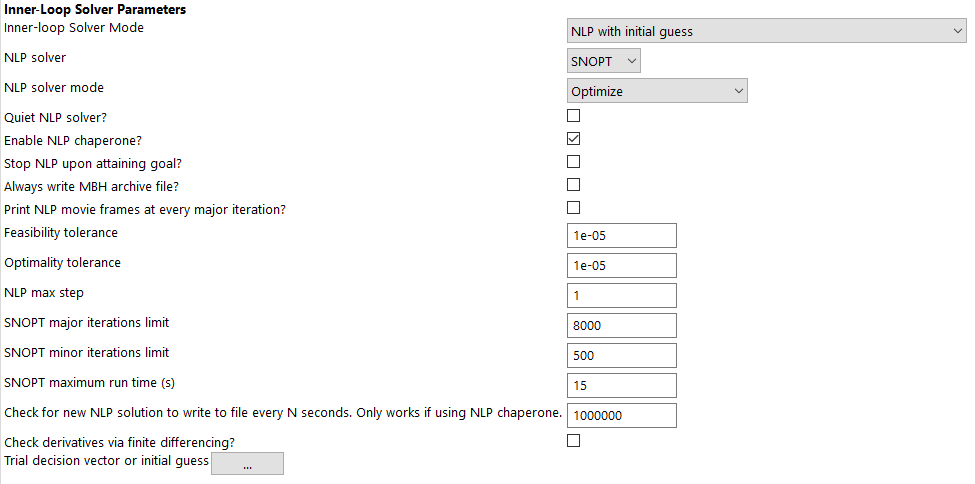
\includegraphics[width=0.7\linewidth]{Testatron_OSIRIS-REx_solver_options.png}}
	\caption{\label{fig:solver_options}OSIRIS-REx\_testatron Solver Options.}
\end{figure}

	\item Update the path to the working directory so that output will go into the new folder. Then, run the Mission using PyEMTG (File-\textgreater Run or Ctrl+r).

Now that *.emtgopt and *.emtg files have been generated, they need to be placed into the correct Testatron test folder. Imagine that the OSIRIS-REx\_testatron.emtgopt file was using a new feature in the Solver Options tab. In this case, the new test would go in the ``solver\_options'' folder in the Testatron tests directory. 

	\item Copy the *.emtgopt and *.emtg files files into \textless EMTG\_root\_dir\textgreater\textbackslash testatron\textbackslash tests\textbackslash solver\_opti-\newline\indent ons.

NOTE: You should not copy tests into the ``tests\_that\_dont\_work'' folder as this folder is for tests that are expected to fail with the current build of \ac{EMTG}.

	\item Copy the OSIRIS-REx mission default.emtg\_spacecraftopt and default.emtg\_propulsionsystem-\indent opt files from the OSIRIS-REx hardware\_models folder into the \textless EMTG\_root\_dir\textgreater\textbackslash testatron\textbackslash{} HardwareModels folder. All other required files in the hardware\_models folder and the Universe folder are already in the corresponding Testatron folders.

NOTE: There is no need to change the paths to ``hardware\_models'' or the Universe folder in the *.emtgopt file, because Testatron will do this automatically.\knownissuelabel{However, if you use a *.emtg\_spacecraftopt or *.emtg\_propulsionsystemopt file that contains a path to another file, such as a *.ThrottleTable file, this path will need to be updated manually within the spacecraft or propulsion system options file.}{hardware_options_file_paths_issue}

\end{enumerate}

%%%%%%%%%%%%%%%%%%%%%
\subsection{Running the New Test}
\label{sec:running_the_new_test}
%%%%%%%%%%%%%%%%%%%%%

Now that all the required files are added, the new test can be run using the run test case command:

\texttt{python testatron.py --emtg <EMTG\_root\_dir>\textbackslash bin\textbackslash EMTGv9.exe --pyemtg <EMTG\_root\_\newline\indent dir>\textbackslash PyEMTG\textbackslash{} -c <EMTG\_root\_dir>\textbackslash testatron\textbackslash tests\textbackslash solver\_options\textbackslash OSIRIS-REx\_test\newline\indent atron}

\noindent The test should run quickly, but you will notice that it fails on the initial run as shown in Figure \ref{fig:osiris_testatron_initial_run}.

\noindent\knownissuelabel{NOTE: This failure is due to Testatron slightly changes some of the numbers used in the OSIRIS-REx\_testatron.emtgopt file, which causes \ac{EMTG} to produce slightly different results. This is likely occurring from number to string conversions in python. A bug ticket has been created for this.}{testatron_changes_emtgopt_issue}

\begin{figure}[H]
	\centering
	\fbox{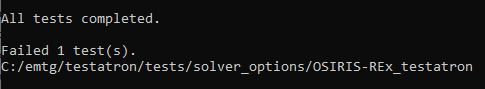
\includegraphics[width=0.6\linewidth]{Testatron_OSIRIS-REx_initial_run.png}}
	\caption{\label{fig:osiris_testatron_initial_run}Initial run output.}
\end{figure}

\noindent To address the slight numerical differences, navigate to the output folder for the test run (located in \textless EMTG\_root\_dir\textgreater\textbackslash testatron\textbackslash output\textbackslash{} \textless time-of-test\textgreater) and copying the OSIRIS-REx\_testatron.emtg file into the solver\_options folder. Run the test again using the same command and it should pass. Example output is shown in Figure \ref{fig:osiris_testatron_success}.

\begin{figure}[H]
	\centering
	\fbox{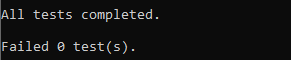
\includegraphics[width=0.5\linewidth]{Testatron_OSIRIS-REx_fixed_run.png}}
	\caption{\label{fig:osiris_testatron_success}Fixed run output.}
\end{figure}

\noindent Congratulations, you have successfully added a test to Testatron and completed the Testatron Tutorials!


\end{document}